\documentclass[11pt,aspectratio=169]{beamer}

\usetheme{metropolis}
\usecolortheme{default}
\metroset{numbering=fraction, progressbar=frametitle, sectionpage=none}

\setbeamertemplate{navigation symbols}{}
\setbeamercolor{frametitle}{bg=mDarkTeal, fg=white}
\setbeamercolor{progress bar}{fg=mDarkTeal, bg=mDarkTeal!20}
\definecolor{mDarkTeal}{HTML}{23373B}
\definecolor{mAccent}{HTML}{EB811B}

\usepackage{amsmath,amssymb}
\usepackage{graphicx}
\usepackage{booktabs}
\usepackage{appendixnumberbeamer}

\title{Math Bootcamp}
\subtitle{Day 3 --- Remaining real analysis and linear algebra}
\author{Math Camp 2026}
\date{}

\newcommand{\InterestOnly}{\textcolor{mAccent}{\textbf{for interest only}}}

\begin{document}

\begin{frame}
  \titlepage
\end{frame}

\begin{frame}{How to use these slides}
  \small
  \textbf{Main deck:}\ definitions, recipes, examples, and practice.

  \medskip
  \textbf{Appendix and proofs} (marked on relevant slides):\
  \InterestOnly\ --- optional recap for those already comfortable with the math.

  \medskip
  \textbf{Not required for Math Camp.}\
  Focus on the main slides and exercises unless you want the extra detail.
\end{frame}

\section{3.1 --- Fixed Point Theorems}

\begin{frame}{3.1 Fixed points --- equilibrium as a solution}
  \footnotesize
  \textbf{Fixed point.}\ A point $x^*$ is a \textbf{fixed point} of a map $T$ if $T(x^*)=x^*$.

  \medskip
  \textbf{Economics reading.}\ Many equilibria are fixed-point problems:
  \begin{itemize}
    \item \textbf{Market clearing:}\ a price $p^*$ with excess demand $E(p^*)=0$.
    \item \textbf{Game theory:}\ a strategy profile that is a best response to itself (Nash).
  \end{itemize}

  \medskip
  \textbf{Two useful existence tools (today).}
  \begin{itemize}
    \item \textbf{Contraction Mapping Theorem:}\ existence and uniqueness of a fixed point; iteration converges.
    \item \textbf{Brouwer:}\ continuous map on a closed interval / convex set.
  \end{itemize}
\end{frame}

\begin{frame}{3.1 Contraction Mapping Theorem}
  \footnotesize
  \textbf{Contraction.}\ A map $T$ \textbf{shrinks distances} if there is $k\in(0,1)$ such that
  $|T(x)-T(y)|\le k|x-y|$ for all $x,y$ in the domain.

  \medskip
  \textbf{Contraction Mapping Theorem.}\ If $T\colon[a,b]\to[a,b]$ is a contraction, then
  \begin{itemize}
    \item \textbf{Existence:}\ there is a fixed point $x^*$ with $T(x^*)=x^*$.
    \item \textbf{Uniqueness:}\ that fixed point is \textbf{unique}.
    \item \textbf{Iteration:}\ for any starting value $x_0\in[a,b]$, the sequence
      $x_n=T(x_{n-1})$ converges to $x^*$.
  \end{itemize}
\end{frame}

\begin{frame}{3.1 Why iteration converges}
  \footnotesize
  \textbf{Step 1 --- Start anywhere.}\
  Pick any $x_0$. Define $x_n=T(x_{n-1})$ for $n=1,2,\ldots$

  \medskip
  \textbf{Step 2 --- Jumps shrink exponentially.}\
  Each new step is at most $k$ times the previous jump:
  \[
    |x_{n+1}-x_n|=|T(x_n)-T(x_{n-1})|\le k|x_n-x_{n-1}|\le k^n|x_1-x_0|.
  \]
  Since $k<1$, the moves get \textbf{exponentially smaller} --- the path barely changes after a while.

  \medskip
  \textbf{Step 3 --- The sequence converges.}\
  Step~2 implies $x_n\to x^*$ for some limit $x^*$
  (check it is a \textbf{Cauchy sequence} for a rigorous proof).
  So iteration from \textbf{any} starting point drives $x_n$ toward the same $x^*$.

  \medskip
  \textbf{Step 4 --- The limit is a fixed point.}\
  $T$ is continuous, so taking limits in $x_n=T(x_{n-1})$ gives
  $x^*=\lim x_n=\lim T(x_{n-1})=T(\lim x_{n-1})=T(x^*)$.
\end{frame}

\begin{frame}{3.1 Walrasian price adjustment}
  \footnotesize
  \textbf{Market clearing.}\ A price $p^*$ \textbf{clears the market} when excess demand is zero:
  $E(p^*)=0$.
  Here $E(p)$ can take \textbf{any form} (from supply and demand behind the scenes).

  \medskip
  \textbf{Price adjustment (nonlinear in $E$).}\ Update the price each period:
  \[
    p_{t+1}=T(p_t)=p_t+\lambda\bigl(1-e^{-\alpha E(p_t)}\bigr),
    \qquad \lambda=\tfrac{1}{5},\ \alpha=0.1.
  \]
  When $|E|$ is small, $1-e^{-\alpha E}\approx \alpha E$ --- move a fraction of excess demand toward balance.
  Clearing satisfies $E(p^*)=0\ \Leftrightarrow\ T(p^*)=p^*$.
  If $T$ is a \textbf{contraction} on a price range, then $p_t\to p^*$ from any starting $p_0$.
\end{frame}

\begin{frame}{3.1 Brouwer --- one dimension}
  \footnotesize
  \textbf{Brouwer (one dimension).}\ If $T\colon[a,b]\to[a,b]$ is \textbf{continuous}, then
  $T$ has \textbf{at least one} fixed point $x^*$ with $T(x^*)=x^*$.

  \medskip
  \textbf{Picture.}\ Plot $y=T(x)$ against $y=x$. Any crossing is a fixed point.
  Continuity forces the graph to meet the diagonal at least once on $[a,b]$.
\end{frame}

\begin{frame}[plain]{}
  \centering
  \vspace{-0.15cm}
  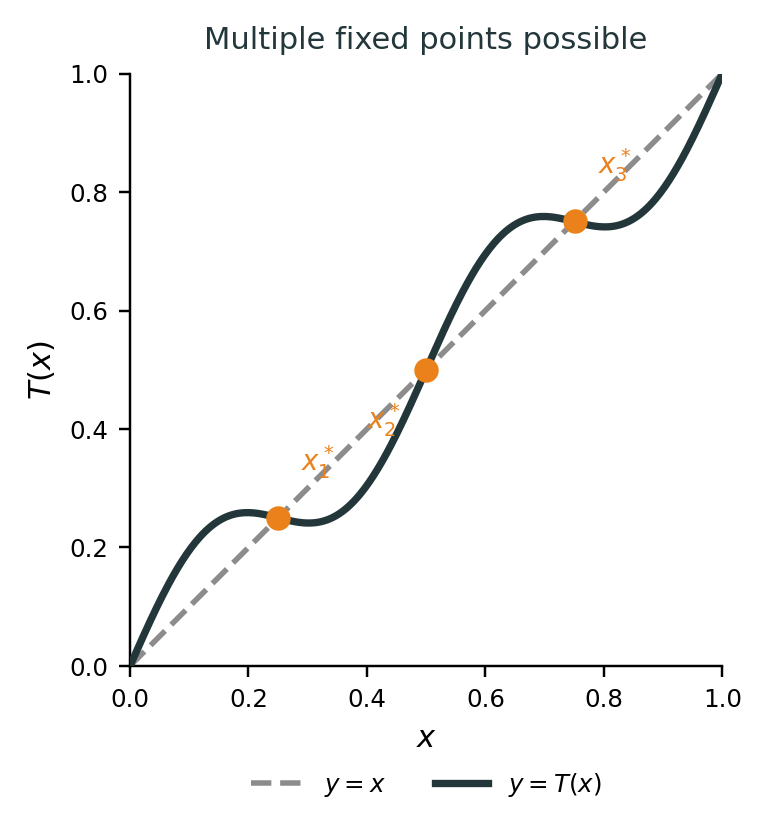
\includegraphics[width=0.88\textwidth,height=0.92\textheight,keepaspectratio]{figures/fixed_point_brouwer.png}
\end{frame}

\begin{frame}{3.1 Brouwer --- general statement}
  \footnotesize
  \textbf{Brouwer (several variables).}\ Let $K\subset\mathbb{R}^n$ be \textbf{nonempty},
  \textbf{compact}, and \textbf{convex}. If $T\colon K\to K$ is \textbf{continuous}, then
  $T$ has at least one fixed point $x^*\in K$ with $T(x^*)=x^*$.

  \medskip
  \textbf{Camp vocabulary.}
  \begin{itemize}
    \item \textbf{Compact} in $\mathbb{R}^n$: closed and bounded (Heine--Borel).
    \item \textbf{Convex}: the segment between any two points in $K$ stays in $K$.
  \end{itemize}

  \medskip
  \textbf{One dimension.}\ $K=[a,b]$ is compact and convex, so the 1D case is a special case.
\end{frame}

\begin{frame}{3.1 Brouwer --- Cournot duopoly}
  \footnotesize
  \textbf{Two firms.}\ Firm $i$ chooses $q_i\in[0,\bar q]$.
  \textbf{Nonlinear} inverse demand $p=a-(q_1+q_2)^2$ (e.g.\ $a=8$, $\bar q=2$).

  \medskip
  \textbf{Profit and FOC.}\ $\pi_i=(a-(q_1+q_2)^2)q_i$. Firm~1's best response solves
  \[
    a-3q_1^2-4q_1 q_2-q_2^2=0
    \qquad\text{(similarly for firm~2 with $q_1,q_2$ swapped).}
  \]
  The map $q_j\mapsto BR_i(q_j)$ is \textbf{nonlinear} --- no formula like
  ``$(a-c-q_j)/2$''.

  \medskip
  \textbf{Fixed point = Nash.}\ $T(q_1,q_2)=\bigl(BR_1(q_2),BR_2(q_1)\bigr)$ is continuous on
  $K=[0,\bar q]^2$. \textbf{Brouwer} guarantees an equilibrium, but you generally solve
  $T(q_1^*,q_2^*)=(q_1^*,q_2^*)$ by \textbf{algebra or numerics}
  (here one symmetric solution is $q_1^*=q_2^*=\sqrt{a/8}$).
\end{frame}

\section{3.2 --- Separation Theorem}

\begin{frame}[plain]{3.2 Separation --- picture}
  \centering
  \vfill
  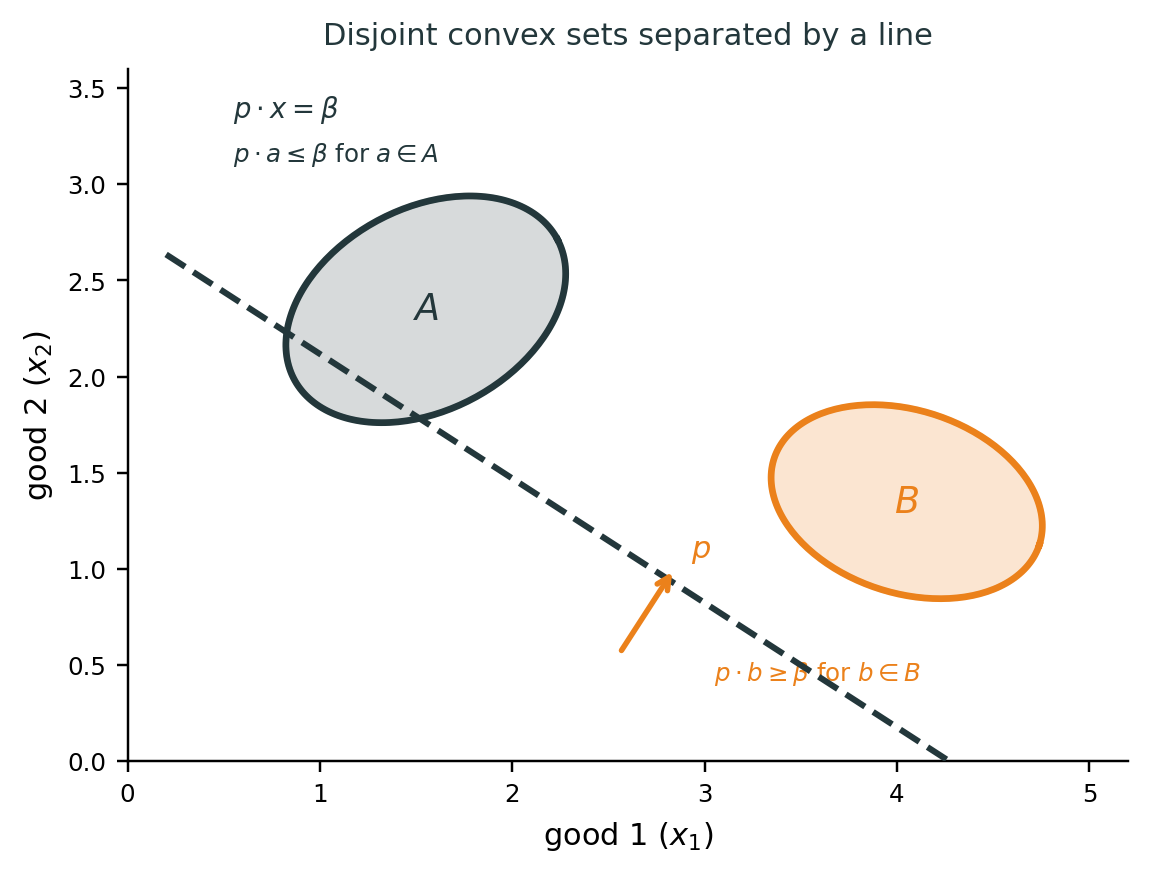
\includegraphics[width=0.78\textwidth]{figures/separation_hyperplane.png}
  \vfill
\end{frame}

\begin{frame}{3.2 What $\mathbf{p}\cdot a\le\beta\le\mathbf{p}\cdot b$ means}
  \footnotesize
  \textbf{Two dimensions, two goods.}\ Write a bundle as $a=(a_1,a_2)$.
  A \textbf{price line} is
  \[
    p_1 x_1 + p_2 x_2 = \beta
    \qquad\text{(same as }\mathbf{p}\cdot x=\beta\text{)}.
  \]

  \medskip
  \textbf{Reading the inequalities.}
  \begin{itemize}
    \item $\mathbf{p}\cdot a\le\beta$ for all $a\in A$: every point of $A$ lies on the
      \textbf{same side} of the line (here: on or below it).
    \item $\mathbf{p}\cdot b\ge\beta$ for all $b\in B$: every point of $B$ lies on the
      \textbf{opposite side} (here: on or above it).
  \end{itemize}

  \medskip
  So $A$ and $B$ are \textbf{separated} by one straight line; $\mathbf{p}$ is the slope/normal of that line,
  and $\beta$ fixes its position. No matrices needed --- just prices and a budget line.
\end{frame}

\begin{frame}{3.2 Example --- feasible vs.\ preferred bundles}
  \footnotesize
  \textbf{Setup.}\ One consumer, two goods. Let
  \begin{itemize}
    \item $A$ = \textbf{feasible} bundles (can be produced / afforded at given resources);
    \item $B$ = bundles \textbf{strictly preferred} to the status quo (better indifference curves).
  \end{itemize}
  If preferences are convex, $B$ is convex. If $A\cap B=\varnothing$, a separating line exists.

  \medskip
  \textbf{Numerical sketch.}\ Suppose the line is $p_1 x_1 + p_2 x_2 = 100$ with $\mathbf{p}=(2,5)$.
  \begin{itemize}
    \item Feasible bundle $a=(10,16)$: $2\cdot10+5\cdot16=100$ --- on the line (cheapest feasible choice).
    \item Preferred bundle $b=(14,18)$: $2\cdot14+5\cdot18=118>100$ --- above the line, not affordable at these prices.
  \end{itemize}

  \medskip
  At a competitive allocation, a price line can sit between ``what is possible'' and ``what everyone wants more of.''
\end{frame}

\begin{frame}{3.2 First Welfare Theorem --- simple argument}
  \footnotesize
  \textbf{Statement.}\ Under standard convexity, a competitive equilibrium allocation is \textbf{Pareto efficient}.

  \medskip
  \textbf{Proof idea (4 steps).}
  \begin{enumerate}
    \item In equilibrium, each consumer chooses a best affordable bundle; each firm maximizes profit at prices $\mathbf{p}^*$.
    \item Suppose another allocation $\tilde x$ is Pareto better: everyone weakly better off, someone strictly.
    \item With convex preferences, if $\tilde x$ were affordable at $\mathbf{p}^*$, some agent would have chosen it --- contradiction.
    \item So any Pareto improvement must use bundles that are \textbf{not affordable} at $\mathbf{p}^*$: the aggregate ``better than'' set
      lies on the expensive side of the equilibrium price line, while feasible aggregates stay on the cheap side.
      \textbf{Separation} is exactly the geometry behind step 4.
  \end{enumerate}
\end{frame}

\begin{frame}{3.2 Duality and separation}
  \footnotesize
  \textbf{Primal problem (example).}\ ``Choose $x$ to maximize utility subject to a budget / resource constraint.''
  \[
    \max u(x)\quad\text{s.t.}\quad \mathbf{p}\cdot x \le w.
  \]

  \medskip
  \textbf{Dual side.}\ The prices $\mathbf{p}$ and cutoff $\beta$ in
  $\mathbf{p}\cdot x\le\beta$ are \textbf{shadow values}:
  \begin{itemize}
    \item they tell how much one unit of each good ``costs'' at the margin;
    \item in constrained optimization, Lagrange multipliers play the role of $\mathbf{p}$;
    \item a \textbf{separating line} is the same object: coefficients $\mathbf{p}$ and level $\beta$ that
      separate feasible from preferred points.
  \end{itemize}

  \medskip
  \textbf{Link.}\ Separation $\Leftrightarrow$ existence of prices supporting an efficient allocation
  $\Leftrightarrow$ dual variables in the primal problem. Day~4--5 make this algorithmic (LP, KKT).
\end{frame}

\end{document}
